\documentclass[../seminar.tex]{subfiles}
\begin{comment}


\documentclass{ferseminar}
\usepackage{subfiles}
\usepackage[bottom]{footmisc}
\usepackage{graphicx}
\usepackage{caption}
\usepackage{subcaption}
\graphicspath{{../Slike/}}
\end{comment}

\begin{document}

Ultra širokokutnim objektivom smatraju se svi objektivi koji sadrže sustav leća žarišne duljine značajno manje od uobičajene čime se postiže široko vidno polje (obično se sve oko i iznad 180° smatra ultra širokim). Takvi objektivi se nazivaju "ribljim okom" (engl. \textit{fisheye\footnote{Sam termin \textit{fisheye} je osmislio početkom 20. st. američki fizičar Robert W. Wood koji se bavio modeliranjem pretpostavke kako ribe vide pod vodom.} lens}) prvenstveno zbog svojeg specifičnog ispupčenog izgleda koje podsjeća na riblje oko (Slika \ref{fig:fisheye_primjeri} (a) ). Najveći nedostatak takvih objektiva je prepoznatljivo vrlo jako radijalno izobličenje (Slika \ref{fig:fisheye_primjeri} (b) ). Razumijevanjem uzroka izobličenja odnosno modela stvaranja slike u kamerama s ribljim okom moguće je navedeno izobličenje ispraviti.

\begin{figure*}[ht!]
    \centering
    \begin{subfigure}[t]{0.5\textwidth}
        \centering
        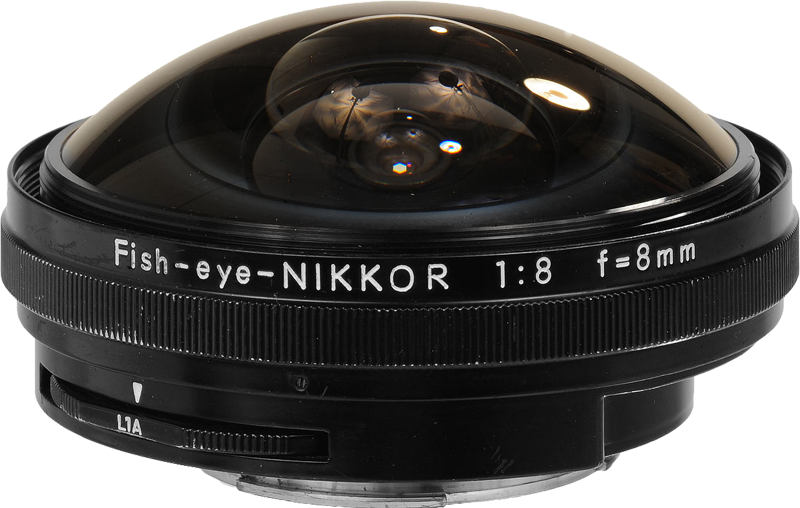
\includegraphics[height=1.5in]{img_001_fisheye_lens_02.png}
        \caption{Riblje oko}
    \end{subfigure}%
    ~ 
    \begin{subfigure}[t]{0.5\textwidth}
        \centering
        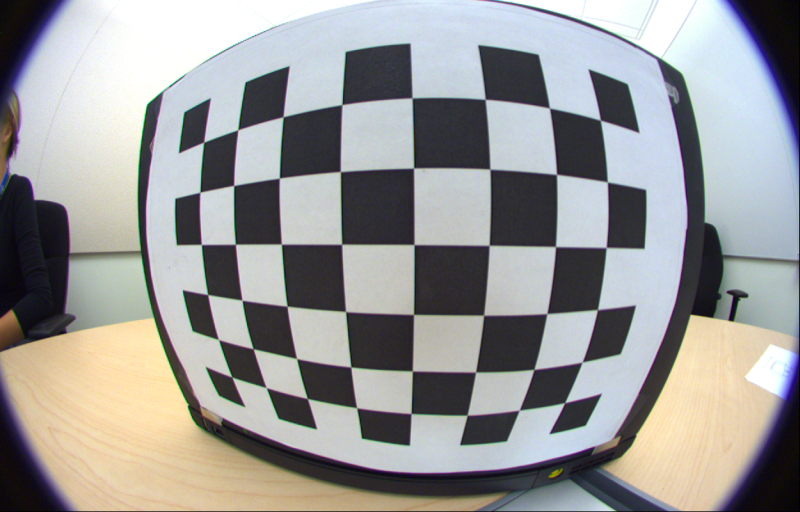
\includegraphics[height=1.5in]{img_002_fisheye_image_01.png}
        \caption{Slika nastala pomoću kamere s ribljem okom}
    \end{subfigure}
    \caption{Primjer ribljeg oka (izvor: \cite{KenRockwell:Nikon}) i slike nastale ribljim okom (izvor: \cite{Kashyap})}
    \label{fig:fisheye_primjeri}
\end{figure*}

\subsection{Perspektivni model stvaranja slike}
Tipična perspektivna kamera može preslikavati točke u uskom polju vidnog polja ispred ravnine slike kamere. 
Neka je $\theta$ kut između glavne (engl. \textit{principal axis}) osi i upadajuće zrake (Slika \ref{fig:perspektivni_model}).
Tada se perspektivna projekcija kamere s infinitezimalnim (točkastim) otvorom (engl. \textit{pin-hole camera}) može opisati na sljedeći način:
\begin{equation}
r = f tan(\theta)
\end{equation}

$O$ je ishodište koordinatnog sustava slike (engl. \textit{principal point}) koja je sjecište glavne osi i ravnine slike. 
$f$ je žarišna duljina (engl. \textit{focal length}), a $r$ je udaljenost između točke slike i ishodišta k.s. slike. 
Standardni perspektivni model kamere preslikava sve točke scene $M$ u jednu točku $C$ koja se naziva optičkim centrom kamere.
Pravac koji spaja optički centar i točku scene presijeca ravninu slike u 2D točci $m$ koja predstavlja koordinatu slike nastalu preslikavanjem točke $M$. 

Neka je $P \in \mathbb{R}^{3X4}$ matrica projekcije, $M \in \mathbb{R}^4$ homogena točka scene, $m \in \mathbb{R}^3$ homogena točka slike i $\alpha$ skalar.
Tada vrijedi sljedeće:

\begin{equation}
\label{eq:eq2}
\alpha m = PM
\end{equation}

Perspektivni model kamere dekomponira projekcijsku matricu u umnožak matrica kamere, rotacije i translacije.
Matrica kamere predstavlja intrinsične parametre \textbf{$K$}.
Matrica rotacija \textbf{$R$} i matrica translacije \textbf{$t$} (translacija) predstavljaju ekstrinsične parametre kamere.
Koristeći navedene matrice i homogene koordinate jednadžba (\ref{eq:eq2}) se može prikazati na sljedeći način:

\begin{equation}
\alpha m = K[R t]M
\end{equation}

Matrica kamere je matrica dimenzija 3 $\times$ 3 koja sadrži žarišne duljine duž $x$-osi i $y$-osi slike ($f_x$, $f_y$), iskrivljenost (engl. \textit{skew}) $\gamma$ između dvije osi slike i ishodišta k.s. slike ($u_0$,$v_0$):

\begin{equation}
K = \begin{bmatrix}
    f_x     & x_{\gamma}& u_0 \\
    0       & f_y       & v_0 \\
    0       & 0         & 1
\end{bmatrix}
\end{equation}

U ovom modelu možemo predstavljati samo scenu ispred kamere gdje su rubovi ravnine slike granice scene. To ograničava širinu vidnog polja perspektivne kamere\footnote{Perspektivna kamera sadrži svojstvo perspektive (engl. \textit{perspective}) - projekcija na slici objekta koji se nalazi daleko od kamere je manja od projekcije objekta koji se nalazi blizu kamere, objekt se čini manjim od bližeg objekta.} na oko 60°.\cite{Kashyap}

\begin{figure*}[ht!]
    \centering
    \begin{subfigure}[t]{0.5\textwidth}
        \centering
        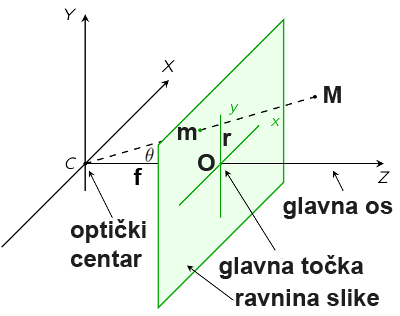
\includegraphics[height=2.2in]{pinhole_camera_model_01.png}
    \end{subfigure}%
    ~ 
    \begin{subfigure}[t]{0.5\textwidth}
        \centering
        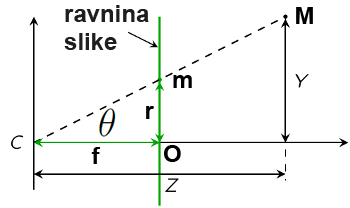
\includegraphics[height=1.5in]{pinhole_camera_model_02.png}
    \end{subfigure}
    \caption{Perspektivni model kamere (izvor: \cite{Chemnitz:Pinhole})}
    \label{fig:perspektivni_model}
\end{figure*}

\clearpage

\subsection{Radijalno simetrični model stvaranja slike}

Perspektivni model stvaranja slike ne odgovara za kamere s ribljim okom. 
Postoje različite vrste kamera s ribljim okom i mogu se se aproksimirati 
pomoću različitih projekcijskih modela. Neka je $r$ radijalna udaljenost piksela od ishodišta k.s. slike, 
$\theta$ kut između upadajuće zrake i optičke osi (Slika \ref{fig:fisheye_model}).
Tada vrijede sljedeći modeli:

\begin{equation}
\label{eq: persp}
r = f tan(\theta)
\end{equation}

\begin{equation}
\label{eq: rad1}
r = 2 f tan(\theta / 2)
\end{equation}

\begin{equation}
\label{eq: rad2}
r = f \theta
\end{equation}

\begin{equation}
\label{eq: rad3}
r = 2f * sin(\theta / 2)
\end{equation}

\begin{equation}
\label{eq: rad4}
r = f sin(\theta)
\end{equation}

Jednadžbe predstavljaju stereografsku projekciju (\ref{eq: rad1}), ekvidistantnu projekciju (\ref{eq: rad2}), ekvisolidnu projekciju (\ref{eq: rad3}) i ortografsku projekciju (\ref{eq: rad4}). Za usporedbu je stavljena jednadžba perspektivne projekcije (\ref{eq: persp}). Primjeri projekcija se mogu vidjeti na Slici (\ref{fig:projekcijski_modeli}).

\begin{figure*}[ht!]
  \centering
    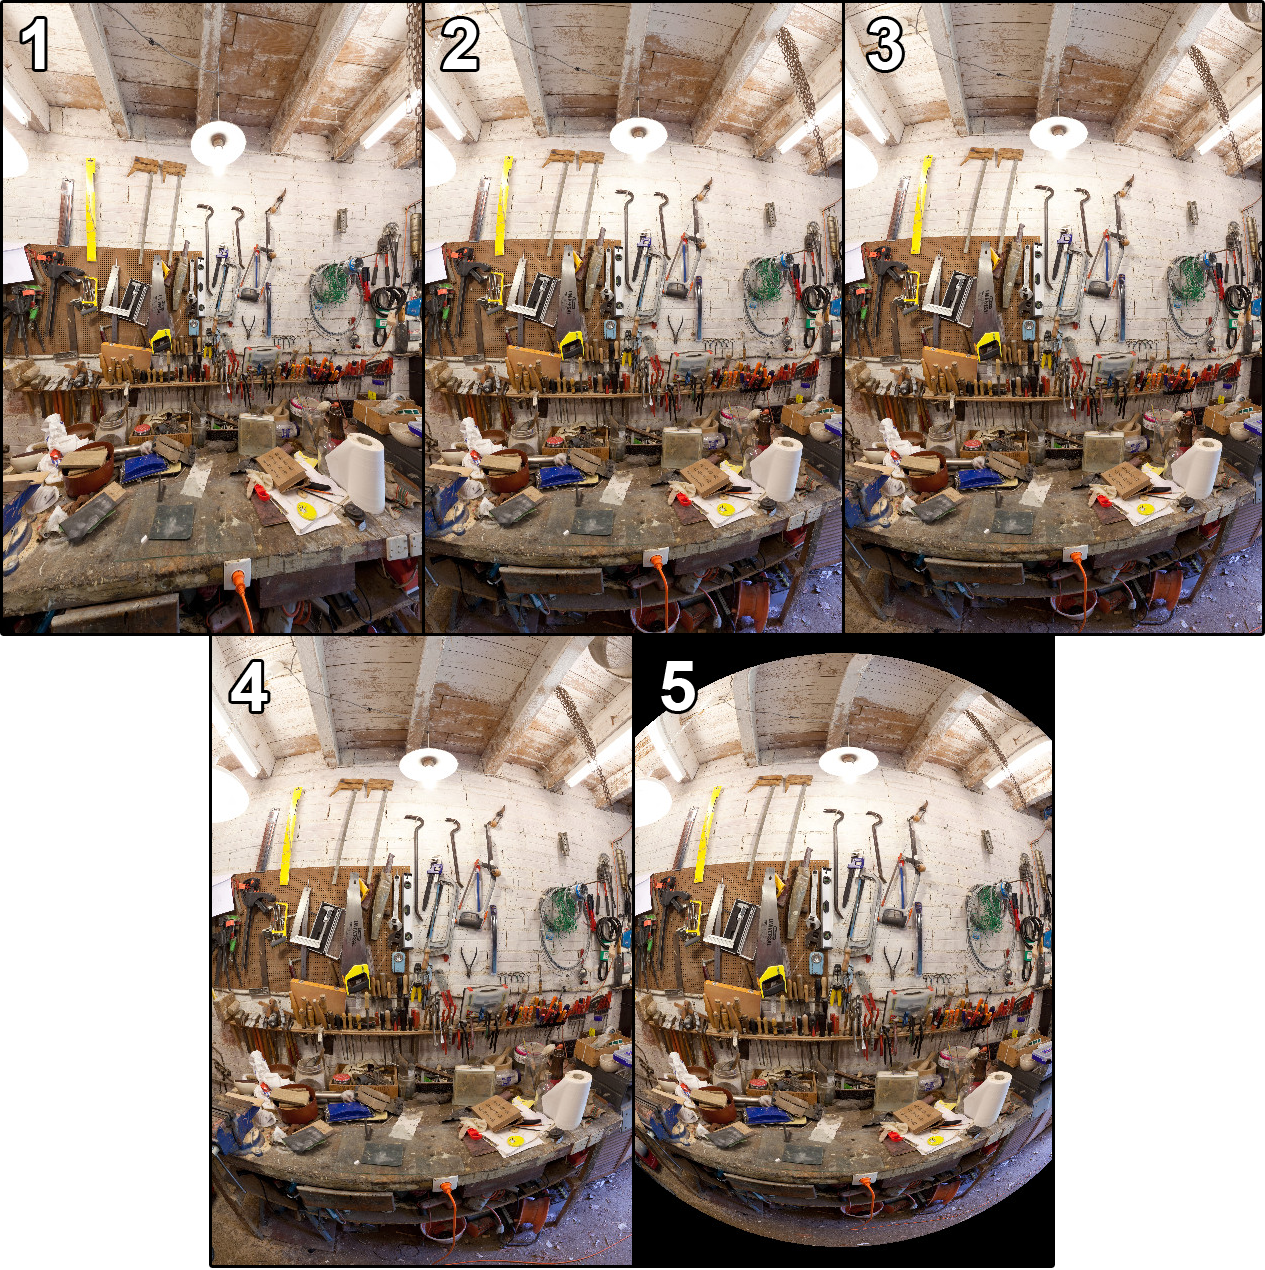
\includegraphics[width=.9\textwidth]{projection_models_examples.png}
   \caption{Primjeri projekcija (izvor: \cite{MichelThoby:Fisheye}): 1 - perspektivna , 2 - stereografska, 3 - ekvidistantna, 4 - ekvisolidna i 5 - ortografska projekcija}
  \label{fig:projekcijski_modeli}
\end{figure*}


Općeniti model kamere s ribljim okom prikazan je slikom \ref{fig:fisheye_model}. 
3D točka prostora $M = [X, Y, Z]$ se preslikava u točku $m = [x, y]$. Također je prikazana točka $m'$ koja prikazuje preslikavanje za perspektivni model. Slično kao i za perspektivne kamere, $\theta$ je kut zrake iz točke $M$ prema centru $C$ s glavnom osi. $O$ je ishodište koordinatnog sustava slike ili centar ravnine slike. Udaljenost između ishodišta k.s. slike  $O$ i točke slike $m$ je radijus $r$. Za radijalne modele vrijedi da je radijus $r$ funkcija kuta $\theta$. 

Time je definiran radijalno simetričan model stvaranja slike no u stvarnosti zbog nesavršene preciznosti izrade leća, a zbog toga i nesavršenosti samih leća, postoje odstupanja od tog modela. Zato je potrebno, osim uzeti u obzir idealni model, obaviti i postupak modeliranja projekcijskog modela za svaku kameru posebno. Taj postupak se naziva kalibracija kamere.
\clearpage

\subsection{Kalibracija kamere s ribljim okom}

Postoje različiti načini kalibracije kamera s ribljim okom. Oni se mogu općenito razvrstati u dvije kategorije: kalibracija pomoću uzorka (engl. \textit{marker-based calibration}) i auto-kalibracija. 

\begin{figure*}[ht!]
  \centering
    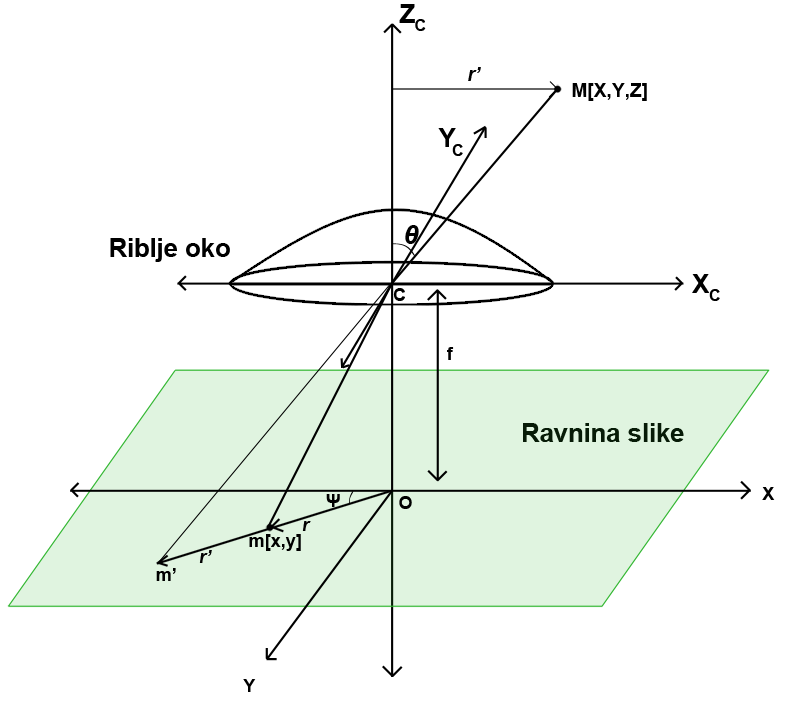
\includegraphics[width=.7\textwidth]{img_003_fisheye_model_01_small.png}
   \caption{Model stvaranja slike pomoću kamere s ribljim okom (izvor: \cite{Kashyap})}
  \label{fig:fisheye_model}
\end{figure*}


\subsubsection{Kalibracija kamera s ribljim okom pomoću uzorka}

Ove metode koriste kalibracijski uzorak i oznake (engl. \textit{markers}) pomoću kojih dobivaju veze između točaka 3D prostora i njihovih projekcija na 2D ravnini slike kamere. Potrebno je koristiti manji broj slika poznatog objekta ili uzorka dobivenih pomoću kamere koja se kalibrira. Poznavajući navedene veze moguće je izračunati funkciju izobličenja (engl. \textit{distortion function}) i druge parametre kamere s ribljim okom. 

Sama kategorija metoda kalibracije pomoću uzorka se može podijeliti na podkategorije ovisno o vrsti korištenog uzorka: kalibracija pomoću 2D uzorka i 3D uzorka. Dvodimenzionalni uzorak koristi 2D planarni uzorak poznate geometrije (poznate su pozicije kontrolnih (specifičnih) točaka i udaljenosti između njih). Najčešće korišteni planarni uzorci su polje ispunjenih kvadrata u obliku šahovnice (Slika \ref{fig: calib_patterns} \subref{fig:calib_patterns_sq}), gdje su kontrolne točke vrhovi kvadrata (Slika \ref{fig: calib_patterns} \subref{fig:calib_patterns_sq_marked}), i polje krugova (Slika \ref{fig: calib_patterns} \subref{fig:calib_patterns_circles}), gdje su kontrolne točke težišta krugova (Slika \ref{fig: calib_patterns} \subref{fig:calib_patterns_circles_marked}). 

\begin{figure*}[ht!]
       \centering
        \begin{subfigure}[b]{0.483\textwidth}
            \centering
            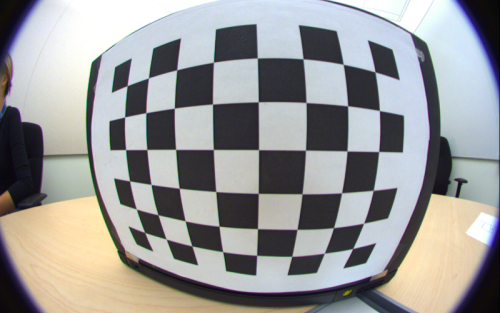
\includegraphics[width=\textwidth]{img_002_fisheye_image_01_small.png}
            \caption[]%
            {{\small Polje ispunjenih kvadrata}}    
            \label{fig:calib_patterns_sq}
        \end{subfigure}
        \hfill
        \begin{subfigure}[b]{0.483\textwidth}  
            \centering 
            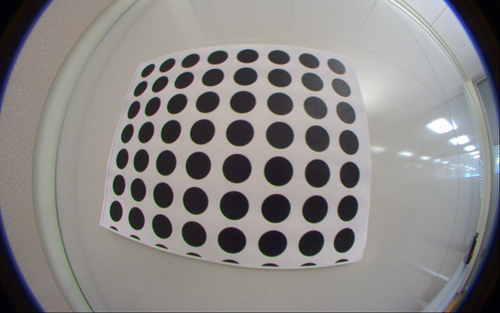
\includegraphics[width=\textwidth]{img_005_calib_circles_01_smaller.png}
            \caption[]%
            {{\small Polje krugova}}    
            \label{fig:calib_patterns_circles}
        \end{subfigure}
        \vskip\baselineskip
        \begin{subfigure}[b]{0.483\textwidth}   
            \centering 
            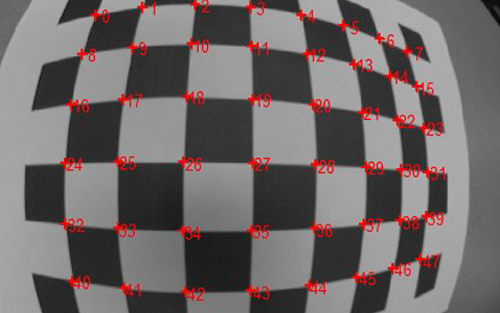
\includegraphics[width=\textwidth]{img_005_calib_sq_marked_01_crop.png}
            \caption[]%
            {{\small Označeni vrhovi kvadrata}}    
            \label{fig:calib_patterns_sq_marked}
        \end{subfigure}
        \quad
        \begin{subfigure}[b]{0.483\textwidth}   
            \centering 
            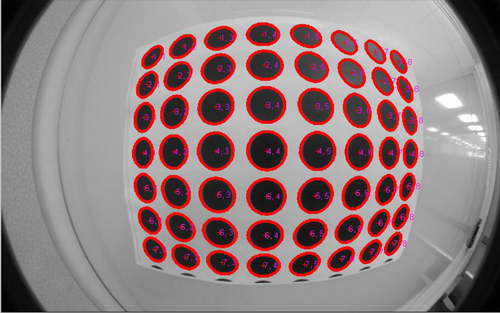
\includegraphics[width=\textwidth]{img_005_calib_circles_marked_01.png}
            \caption[]%
            {{\small Označeni rubovi i težišta krugova}}    
            \label{fig:calib_patterns_circles_marked}
        \end{subfigure}
        \caption[ ]
        {\small Primjeri kalibracijskih uzoraka i njihove oznake (slike s prisutnim izobličenjem) (izvor: \cite{Kashyap})} 
        \label{fig: calib_patterns}
    \end{figure*}

Nakon što je slika uzorka dobivena i kontrolne točke se odrede, izobličenje se modelira na temelju veza između pozicija kontrolnih točaka u slici i poznatih 3D točaka u okolini. Ovo omogućuje estimaciju intrinsičnih parametara kamere.
Slika \ref{fig: calib_3D} prikazuje 3D kalibracijski uzorak. Koristi se metoda diskretne linearne transformacije (DLT) koja zahtijeva samo jednu sliku 3D uzorka. Kao i u planarnom uzorku kontrolne točke su kutovi kvadrata šahovnice na sve tri ravnine. Ovdje se može estimirati homografija između slike uzorka i originalnog kalibracijskog uzorka na temelju kontrolnih točaka. Rezultirajuća homografija  se koristi za kalibraciju kamere i otkrivanje njezinih intrinsičnih parametara.

\begin{figure*}[ht!]
  \centering
    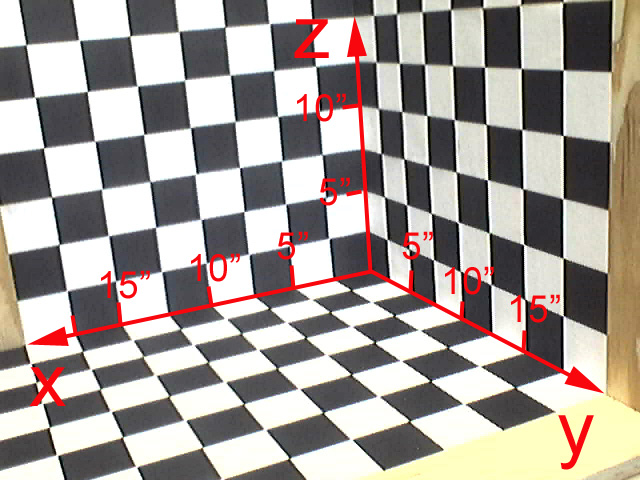
\includegraphics[width=.5\textwidth]{img_006_calib_3D.png}
   \caption{3D kalibracijski uzorak (izvor: \cite{Kashyap})}
  \label{fig: calib_3D}
\end{figure*}
 
\subsubsection{Auto-kalibracija kamera s ribljim okom} 
 
Metode auto-kalibracije se još nazivaju samo-kalibrirajuće metode  jer se kalibracija vrši bez korištenja oznaka čiji je raspored poznat. Takve metode obično zahtijevaju više od jedne slike scene ili neke specifične detalje u strukturi same scene. Određene samo-kalibrirajuće metode koriste samo podudaranja točaka u više pogleda bez potrebe za 3D lokacijama točaka ili pozicija kamere. Kod njih se funkcije izobličenja estimiraju zajedno s ekstrinsičnim parametrima pokreta kamere između slika. Većina tih metoda se temelji na činjenici da centralne kamere podliježu epipolarnoj geometriji. Postoje i samo-kalibrirajuće metode pravaca koje se temelje na detekciji pravaca u sceni. 
One detektiraju zaobljene linije na slici koje odgovaraju ravnim pravcima s poznatim međusobnim udaljenostima. Parametri izobličenja se mogu estimirati pronalaskom transformacije koja najbolje pretvara snimljene zaobljene linije u pravce.  Glavni nedostatak takvih metoda je da se mogu dobiti samo intrinsični parametri kamere jer one ne mogu estimirati ekstrinsične parametre između dva pogleda kamere.
 
\subsubsection{Funkcije izobličenja kamere s ribljim okom}

U praksi se stvaranje slike pomoću kamere s ribljim okom ne podudara s idealnim projekcijskim modelom. Potrebne su dodatne funkcije koje modeliraju već opisano izobličenje. Model radijalnog izobličenja za planarne kamere koristi sljedeće jednadžbe:
\begin{equation}
\label{eq: eq_D_x}
D_x = x_d(k_1r^2 + k_2r^4 + ...)
\end{equation}
\begin{equation}
\label{eq: eq_D_y}
D_y = y_d(k_1r^2 + k_2r^4 + ...)
\end{equation}
\begin{equation}
r = \sqrt{x_d^2 + y_d^2}
\end{equation}

$(x_d, y_d)$ su koordinate izobličenje slike, $r$ je radijalna udaljenost između centra i piksela izobličene slike i $(D_x, D_y)$ su izobličenja (engl \textit{distortions}) u smjeru X i Y-osi. U nekim postupcima se koristi samo jedan koeficijent $k_1$ u jednadžbama \ref{eq: eq_D_x} i \ref{eq: eq_D_y}, ali time se mogu modelirati samo manja izobličenja za planarne kamere, ali ne i za kamere s ribljim okom zbog velikog radijalnog pomaka. 
\clearpage

Postoje funkcije izobličenja razvijene posebno za kamere s ribljim okom:

\begin{itemize}
\setlength\itemsep{2em}
\item \textbf{Polinomni model ribljeg oka}
\begin{equation}
\theta = \sum\limits_{i=1}^\infty k_n r^n = k_1 r + k_2 r^2 + ...
\end{equation}
$r$ je radijalna udaljenost od ishodišta k.s. slike (centra slike) i $\theta$ je kut između upadajuće zrake i optičke osi (Slika \ref{fig:fisheye_model}). Za simuliranje izobličenja leća ribljeg oka smatra se adekvatnim korištenje četvrtog reda modela.

\item \textbf{Model vidnog polja FOV (engl. \textit{Field Of View model})}
\begin{equation}
r_d = \frac{1}{\omega}tan^{-1}(2r_u tan(\frac{\omega}{2}))
\end{equation}
$\omega$ je vidno polje kamere u radijanima, $r_d$ je radijalna udaljenost od glave točke u izobličenoj slici i $r_u$ je radijalna udaljenost od ishodišta k.s. slike u planarnoj slici. FOV model se temelji na jednostavnom optičkom modelu kamere s ribljim okom.

\item \textbf{Transformacija ribljeg oka (engl \textit{fisheye transform})}
\begin{equation}
r_d = s * ln(1 + \lambda r_u)
\end{equation}
$s$ je skalar, a $\lambda$ kontrolira količinu izobličenja.

\item \textbf{Model diobe (engl \textit{division model})}
\begin{equation}
r_d = \frac{(l + 1)\sin \theta}{l + \cos \theta}
\end{equation}
$\theta$ je kut između upadajuće zrake i optičke osi kamere (Slika \ref{fig:fisheye_model}), a $l$ parametar izobličenja.
\end{itemize}


\end{document}
